\documentclass[10pt,twocolumn,letterpaper]{article}

% สิ่งที่ฉันเพิ่มเอง
\usepackage{booktabs}
% \usepackage{caption}
% \captionsetup[table]{skip=8pt}   % มีผลเฉพาะกับตาราง
\usepackage{stfloats}  % เพิ่มอันนี้ใน preamble
\usepackage{float}
\usepackage[T1]{fontenc}

\XeTeXlinebreaklocale "th"
\XeTeXlinebreakskip = 0pt plus 1pt

\usepackage{fontspec}
\usepackage{ucharclasses}

%–– define your two fonts ––
\newfontfamily\latinfont{Latin Modern Roman}      % for all non-Thai text
\newfontfamily\thaifont[Script=Thai]{FreeSerif}    % for all Thai text

%–– ucharclasses auto-detects Unicode blocks ––
\setDefaultTransitions{\latinfont}{}              % outside Thai → Latin
\setTransitionsFor{Thai}{\thaifont}{\latinfont}   % Thai block → Thai font, then back

\usepackage{cvpr}
\usepackage{times}
\usepackage{epsfig}
\usepackage{graphicx}
\usepackage{amsmath}
\usepackage{amssymb}


\usepackage[breaklinks=true,bookmarks=false]{hyperref}
\cvprfinalcopy % *** ยกเลิกคอมเมนต์บรรทัดนี้สำหรับการส่งต้นฉบับฉบับสุดท้าย

\makeatletter
\def\cvprsubsection{\@startsection {subsection}{2}{\z@}
    {8pt plus 2pt minus 2pt}{6pt}{\bfseries\normalsize}}
\makeatother


\def\cvprPaperID{****} % *** ใส่รหัสประจำตัวกระดาษ CVPR ที่นี่
\def\httilde{\mbox{\tt\raisebox{-.5ex}{\symbol{126}}}}

% 1) Choose your desired fixed leading:
\renewcommand\baselinestretch{1.2}  % or 1.3, 1.1…  adjust to taste

% 2) Force TeX to *always* use \baselineskip, never fall back to \lineskip:
\makeatletter
  \setlength\lineskiplimit{-\maxdimen} % always allow baselineskip
  \setlength\lineskip{0pt}             % no extra glue ever
\makeatother


\renewcommand{\tablename}{ตาราง}
\renewcommand{\figurename}{รูปที่}   % or whatever you like instead of "Hình"
\renewcommand{\refname}{เอกสารอ้างอิง}

\makeatletter
\def\abstract{%
  \centerline{\large\bf บทคัดย่อ}% <-- your new label
  \vspace*{12pt}%
  \it%
}
\renewcommand\endabstract{%
  \vspace*{0pt}% cut this in half
}
\makeatother

% This makes the font slightly bigger than base (10) and bold in Subsection headings rather than using ptmb
\makeatletter
\def\cvprsubsection{%
  \@startsection{subsection}{2}{\z@}%
    {8pt plus 2pt minus 2pt}{6pt}%
    % {\normalfont\bfseries\selectfont}%
    {\normalfont\bfseries\fontsize{11}{13}\selectfont}%
}
\makeatother

% So this hardcodes the style for the numbers in the section/subsection headings so they're bold
\font\elvbf=ptmb scaled 1100
\font\elvbfs=ptmb scaled 1200
\makeatletter
% Section number: Large + bold
\renewcommand\thesection{%
  {\elvbfs\arabic{section}}%
}

% Subsection number: normalsize + bold + custom punctuation
\renewcommand\thesubsection{%
  {\elvbf
   \arabic{section}.\arabic{subsection}}%
}
\makeatother

% หน้าถูกนับเลขในโหมดส่งต้นฉบับ และไม่มีเลขหน้าในฉบับกล้องพร้อมพิมพ์
%\ifcvprfinal\pagestyle{empty}\fi
\setcounter{page}{1}
\begin{document}

%%%%%%%%% TITLE
\title{เอกสารแนะนำทฤษฎีECDOที่ขับเคลื่อนโดยข้อมูล  ตอนที่ 1/2: ความเข้าใจปัจจุบันเกี่ยวกับการแยกตัวของแก่นโลกและเนื้อโลกซึ่งเป็นกระบวนการคายความร้อน ทำให้เกิดการแกว่งในลักษณะจานิเบคอฟในการหมุนของโลก  (ECDO) ทฤษฎี"การพลิกสลับขั้วแม่เหล็กโลก"}

\author{จุนโฮ\\
เผยแพร่ กุมภาพันธ์ 2025\\
เว็บไซต์ (ดาวน์โหลดเอกสารที่นี่): \href{https://sovrynn.github.io}{sovrynn.github.io}\\
คลังข้อมูลวิจัย ECDO: \href{https://github.com/sovrynn/ecdo}{github.com/sovrynn/ecdo}\\
{\tt\small junhobtc@proton.me}
}
\maketitle
%\thispagestyle{empty}

\begin{abstract}
ในเดือนพฤษภาคม ค.ศ. 2024  นักเขียนออนไลน์ผู้ใช้นามแฝงชื่อว่า “The Ethical Skeptic” \cite{0} ได้เผยแพร่ทฤษฎีใหม่เรียกว่า Exothermic Core-Mantle Decoupling Dzhanibekov Oscillation การแยกตัวของแก่นโลกและเนื้อโลกซึ่งเป็นกระบวนการคายความร้อน ทำให้เกิดการแกว่งในลักษณะจานิเบคอฟในการหมุนของโลก (ECDO) \cite{1} ทฤษฎีนี้เสนอว่า โลกเคยประสบกับการเปลี่ยนแปลงแกนหมุนอย่างกะทันหันจนอาจทำให้เกิดน้ำท่วมโลกขึ้น เพราะทะเลหลากล้นแผ่นดินเนื่องด้วยแรงเฉื่อยการหมุนของโลก นอกจากนี้ ยังมีการนำเสนอกระบวนการทางธรณีฟิสิกส์และข้อมูลที่บ่งชี้ว่า การสลับขั้วเช่นนี้อาจเกิดขึ้นอีกในไม่ช้า แม้การทำนายเหตุการณ์น้ำท่วมโลกและวันโลกาวินาศจะไม่ใช่เรื่องใหม่ แต่ทฤษฎี ECDO มีความน่าสนใจอย่างยิ่งเนื่องจากใช้วิธีการทางวิทยาศาสตร์ สมัยใหม่ สหสาขาวิชาชีพ และอ้างอิงข้อมูลจริง

งานวิจัยนี้เป็นส่วนแรกจากสองตอนจากสารนิพนธ์เป็นเวลา 6 เดือน \cite{2,20} เกี่ยวกับทฤษฎี ECDO ซึ่งจะเน้นประเด็นสำคัญสามข้อดังนี้:

\begin{flushleft}
\begin{enumerate}
    \item ปรากฏการณ์ 'การพลิกสลับขั้วแม่เหล็กโลก' ที่มีลักษณะคล้าย ECDO ได้เกิดขึ้นหลายครั้งในประวัติศาสตร์มนุษย์เมื่อไม่นานมานี้ ดังเห็นได้จากตำนานน้ำท่วมและร่องรอยทางธรณีวิทยาของน้ำท่วมข้ามทวีป
    \item สามารถประมาณทิศทางและขนาดของการสลับขั้วโลกในอดีตได้
    \item ข้อมูลทางสนามแม่เหล็กโลกและธรณีฟิสิกส์ล่าสุดบ่งชี้ว่าการพลิกสลับขั้วแม่เหล็กโลกอาจจะเกิดขึ้นอีกในไม่ช้า และการเปลี่ยนแปลงสภาพภูมิอากาศอาจมีสาเหตุมาจากการเปลี่ยนแปลงภายในใต้ธรณีของโลกมากกว่ากิจกรรมของมนุษย์
\end{enumerate}
\end{flushleft}

นอกจากนี้ ผู้เขียนยังนำเสนอหลักฟิสิกส์ที่เป็นสาเหตุของ “การพลิกสลับขั้วแม่เหล็กโลก” ตามข้อเสนอของทฤษฎี ECDO

ในบทความนี้ ผู้เขียนคงความเป็นกลางโดยเน้นไปที่ข้อมูลจริง หลีกเลี่ยงส่วนที่ดึงดูดแต่ยังคาดเดา และเน้นย้ำว่านี่คือหัวข้อที่มนุษยชาติมีความจำเป็นเร่งด่วนในการค้นคว้าต่อไป
\end{abstract}
\section{บทนำ}

เรื่องราวของน้ำท่วมใหญ่ไม่ใช่เรื่องใหม่ ในความเป็นจริง เรื่องเหล่านี้พบในทุกวัฒนธรรมหลักทั่วโลก ครอบคลุมอารยธรรมดั้งเดิมทั้งหมด จุดใน (รูปที่ \ref{fig:1}) เป็นการรวบรวมเรื่องราวน้ำท่วม 267 เรื่อง \cite{3} แสดงให้เห็นว่าแทบทุกพื้นที่ที่มีผู้คนอยู่อาศัยต่างมีเรื่องเล่าเกี่ยวกับน้ำท่วมทั้งสิ้น

\begin{figure}[b]
\begin{center}
% \fbox{\rule{0pt}{2in} \rule{0.9\linewidth}{0pt}}
   \includegraphics[width=1\linewidth]{b.png}
\end{center}
   \caption{ตำแหน่งของเรื่องเล่าน้ำท่วมทั่วโลก \cite{3}.}
\label{fig:1}
\label{fig:onecol}
\end{figure}

เมื่อลองพิจารณาเรื่องเล่าน้ำท่วมเหล่านี้อย่างใกล้ชิด จะพบว่าเหตุการณ์เหล่านั้นไม่ใช่น้ำท่วมธรรมดา แต่เป็นภัยพิบัติครั้งใหญ่เกิดขึ้นพร้อมกับน้ำท่วมที่กวาดล้างทวีปจนหมดสิ้น

\subsection{เรื่องเล่าภัยพิบัติของชนพื้นเมืองอเมริกัน}

เรื่องเล่าของชนพื้นเมืองอเมริกันมีรายละเอียดเกี่ยวกับภัยพิบัติครั้งใหญ่ของโลกที่ชัดเจนที่สุด ชาวโฮพี ซึ่งเป็นชนพื้นเมืองอเมริกันที่อาศัยอยู่ทางตะวันออกเฉียงเหนือของรัฐแอริโซนา เล่าว่า, \textit{"..โซตุกนัง(Sótuknang) ได้ขอให้มนุษย์มดเปิดโลกใต้ดินของพวกเขาให้กับกลุ่มผู้คนที่ถูกเลือกเมื่อพวกเขาปลอดภัยอยู่ใต้ดินแล้วโซตุกนัง(Sótuknang) ก็สั่งให้ฝาแฝด โปกังโฮย่า( Pöqánghoya) และ
ปาลองกาโวย่า( Palöngawhoya )ออกจากตำแหน่งที่ขั้วเหนือและขั้วใต้ของแกนโลก ซึ่งทั้งสองประจำอยู่เพื่อให้โลกหมุนอยู่ในทิศทางที่ถูกต้อง \textbf{แฝดทั้งสองแทบจะเพิ่งละทิ้งตำแหน่งของตน โลกที่ไม่มีใครควบคุม ทำให้โลกเสียสมดุล หมุนอย่างบ้าคลั่ง แล้วโลกพลิกสองครั้ง} ภูเขาถล่มลงไปในทะเลจนเกิดคลื่นใหญ่ น้ำทะเลและทะเลสาบจึงไหลบ่าท่วมแผ่นดิน และเมื่อตัวโลกหมุนอยู่ในอวกาศที่หนาวเหน็บและไร้สิ่งมีชีวิต ก็แช่แข็งกลายเป็นน้ำแข็ง"} \cite{4}.
เรื่องราวเหล่านี้หลายเรื่องได้บรรยายถึงขนาดอันมโหฬารของน้ำท่วมอย่างละเอียด โดยเล่าว่าทะเลได้ยกตัวสูงขึ้นจนจมหายไปเกือบทุกสิ่งยกเว้นยอดเขาที่สูงที่สุด ชาวอินเดียนสโกโคมิช ซึ่งอาศัยอยู่ในรัฐวอชิงตัน เล่าไว้ว่า \textit{ผู้สร้างสรรค์โลกและสิ่งมีชีวิตทั้งหมดทรงโกรธเคืองความชั่วร้ายของผู้คนและสัตว์ ได้ตัดสินใจล้างโลกโดยให้เหลือแต่สัตว์ที่ดี คนดีหนึ่งคน และครอบครัวของเขาเท่านั้น เมื่อได้รับคำแนะนำจากผู้สร้างสรรค์โลกและสิ่งมีชีวิตทั้งหมดชายผู้นั้นได้ยิงธนูขึ้นไปยังเมฆ จากนั้นก็ยิงอีกลูกเข้าไปในลูกแรก และทำต่อไปเรื่อยๆสร้างเป็นธนูที่ต่อกันเป็นเชือกจากเมฆลงมาถึงพื้นดิน คนและสัตว์ที่ดีได้ปีนขึ้นไป ส่วนสัตว์ที่ชั่วร้ายและงูก็พยายามจะปีนขึ้นไปแต่ชายผู้นั้นได้ทำให้เชือกขาด \textbf{แล้วผู้สร้างสรรค์โลกและสิ่งมีชีวิตทั้งหมดก็ทำให้ฝนตกอยู่นานหลายวัน น้ำท่วมถึงแนวหิมะของทาโคมา (ภูเขาเรนิเยร์)} หลังจากคนและสัตว์ที่ชั่วร้ายจมน้ำตายหมดผู้สร้างสรรค์โลกและสิ่งมีชีวิตทั้งหมดก็หยุดฝน น้ำก็ค่อยๆ ลดลง คนและสัตว์ที่ดีก็ลงมาจากเชือกธนู"} \cite{3} เพื่อประกอบความเข้าใจ ภูเขาเรนิเยร์เป็นภูเขาไฟที่ยังมีพลังในรัฐวอชิงตัน มีความสูงสูงสุด 4,392.5 เมตรจากระดับน้ำทะเล

เรื่องราวน้ำท่วมจากชาวอินเดียนมาคาในรัฐวอชิงตัน ได้พูดถึงน้ำท่วมหลายระยะโดยได้กล่าวถึงระยะที่น้ำ "มีความร้อนมาก" ซึ่งแสดงว่านี่ไม่ใช่น้ำท่วมตามปกติ: \textit{"ทะเลสูงขึ้นมาจนตัดปลายแหลมออก แล้วน้ำก็ลดลงอย่างมากสี่วันต่อมา ทำให้อ่าวเนียห์อยู่เหนือระดับน้ำอย่างสิ้นเชิง จากนั้นน้ำก็สูงขึ้นอีกครั้งจนท่วมเกือบทั้งหมดยกเว้นยอดเขา \textbf{น้ำที่สูงขึ้นมานั้นอุ่นมาก} ผู้คนที่มีเรือแคนูได้บรรทุกสัมภาระของพวกเขาและถูกพัดพาไปไกลทางทิศเหนือ หลายคนเสียชีวิตเมื่อเรือติดกับต้นไม้ ทะเลกลับสู่สภาพปกติหลังจากสี่วันต่อมา และผู้คนพบว่าตนเองไปอยู่ไกลทางเหนือ ซึ่งเป็นที่อาศัยของลูกหลานของพวกเขาจนถึงปัจจุบัน"} \cite{3}

\subsection{เรื่องเล่าเกี่ยวกับภัยพิบัติของประเทศจีน}

อีกฟากฝั่งหนึ่งของมหาสมุทรแปซิฟิก มีการกล่าวว่าระดับอารยธรรมจีนยุคใหม่เริ่มต้นด้วยน้ำท่วมใหญ่ ราชวงศ์เซี่ย ซึ่งคาดว่ามีอยู่ราว 2000 ปีก่อนคริสตกาล ก่อตั้งขึ้นโดยต้าอวี่ ซึ่งหยุดน้ำท่วมใหญ่ของกุ่นอวี่ \cite{6} ในช่วงเวลานั้น \textit{"... มีเรื่องเล่าว่าปาฏิหาริย์เกิดขึ้น ดวงอาทิตย์ไม่ตกดินเป็นเวลาสิบวัน ป่าถูกไฟไหม้ และมีสัตว์ร้ายมากมายเกิดขึ้น ... คลื่นมหึมาที่ 'สูงถึงฟ้า' ซัดถล่มแผ่นดินจีน \textbf{'น้ำสูงขึ้นไปถึงภูเขาสูง ส่วนเชิงเขานั้นจมหายไป'} ... จักรพรรดิตรัสว่า 'น้ำหลากท่วมทำลายล้างอย่างหนัก' 'น้ำกว้างใหญ่ท่วมเนินเขา ท่วมยอดเขาสูงใหญ่ คุกคามสวรรค์ด้วยคลื่นน้ำ' จักรพรรดิทรงมีคำสั่งให้เร่งระดมพลเปิดทางให้น้ำที่ติดอยู่ในหุบเขาระหว่างภูเขาไหลออกไป หลายปีที่ประชาชนพยายามขุดคลองเพื่อระบายน้ำออกจากที่ราบและหุบเขา พยายามอยู่นานหลายปีก็ไม่เป็นผล เสนาบดีที่รับผิดชอบงานสำคัญนี้ชื่อกวานถูกตัดสินประหารชีวิตเพราะล้มเหลว ... และมีเพียงบุตรชายของเขาคืออวี่เท่านั้นที่ประสบความสำเร็จในการระบายน้ำ ความสำเร็จนี้ได้รับการยกย่องสูงจนในที่สุดอวี่ได้เป็นจักรพรรดิของจีนต่อจากกษัตริย์ซุ่น ผู้สืบตำแหน่งคนแรกจากเหยา} \cite{5}

ดูเหมือนว่าไม่เพียงแต่เมืองจีนจะถูกน้ำท่วม ยังต้องมีการวัดทิศหลักและการเคลื่อนที่ของดวงอาทิตย์และดวงจันทร์ใหม่ ซึ่งบ่งชี้ว่าอาจมีการเปลี่ยนแปลงการหมุนของโลกในช่วงน้ำท่วม: \textit{\textbf{"จักรพรรดิตรัสให้บรรดานักปราชญ์เดินทางไปยังภูมิภาคต่างๆ ของจีน แม้กระทั่งอินโดจีน เพื่อหาทิศเหนือ ทิศตะวันตก ทิศตะวันออก และทิศใต้ ด้วยการสังเกตทิศที่ดวงอาทิตย์ขึ้นและตก และการเคลื่อนที่ของดวงดาว} นอกจากนี้ยังให้พระโหราธิบดีค้นหาช่วงเวลาของแต่ละฤดูและจัดทำปฏิทินใหม่ ... 'ต่อมาเหยา ได้ให้เหอกับโหว ปฏิบัติหน้าที่อย่างเคร่งครัดต่อสวรรค์ เพื่อคำนวณและวาดแผนการเคลื่อนไหวและรูปลักษณ์ของดวงอาทิตย์ ดวงจันทร์ ดาว และกลุ่มราศี เพื่อบอกฤดูกาลให้ประชาชนได้รับรู้'"} \cite{5}

บันทึกเกี่ยวกับภัยพิบัติในประวัติศาสตร์จีนมีมาก่อนยุคราชวงศ์เซี่ยเสียอีก โดยย้อนไปถึงยุคสามกษัตริย์ห้าจักรพรรดิ \cite{7} หนี่วา หนึ่งในสามกษัตริย์และเป็นบุคคลสำคัญในตำนานสร้างโลกของจีน ได้หยุดน้ำท่วมในภัยพิบัติที่โลกเปลี่ยนการหมุน: \textit{"มีการทะเลาะกันระหว่างเทพเจ้าสององค์ที่ทรงพลังและพวกเขาตัดสินใจที่จะยุติมันด้วยการต่อสู้ เมื่อเทพเจ้าแห่งน้ำก้งกงเห็นว่าตนเองจะแพ้ ก็เอาหัวโขกภูเขาปูโจว ซึ่งเป็นเสาสวรรค์ที่ค้ำฟ้าอยู่ \textbf{เสาสวรรค์นั้นล้มลงทำให้ท้องฟ้าเอียงไปทางตะวันตกเฉียงเหนือ และแผ่นดินเอียงไปทางตะวันออกเฉียงใต้} ส่งผลให้เกิดภัยพิบัติมากมาย เช่นไฟไหม้ไม่รู้จบ น้ำท่วมใหญ่ และการปรากฏตัวของสัตว์ร้ายที่กินคน หนี่วาตัดขาเต่ายักษ์มาใช้เป็นเสาแทนเสาที่ล่มลง เพื่อลดความรุนแรงของเหตุการณ์ และปิดผนึกท้องฟ้าที่แตกหักโดยใช้หินเจ็ดสี แต่เธอไม่สามารถแก้ไขท้องฟ้าที่เอียงได้อย่างสมบูรณ์"} \cite{8}

\subsection{เรื่องเล่าหายนะในยุโรป มายัน ตะวันออกกลาง และเอเชียตะวันออกเฉียงใต้}

เนื่องจากมีเรื่องเล่าเกี่ยวกับภัยพิบัติมากเกินกว่าที่จะกล่าวถึงทั้งหมดในเอกสารนี้ ขอกล่าวถึงบางวัฒนธรรมสำคัญอื่นๆ ที่มีเรื่องราวเหล่านี้โดยย่อ วรรณกรรมกรีกมีเรื่องราวน้ำท่วมใหญ่สามเรื่องของดีคิวเลียน, ออกิกีส และดาร์ดานัส \cite{9,10} ในเรื่องแรก \textit{"หลังจากน้ำท่วมเก้าวัน โลกถูกทำลาย และเรืออาร์คจอดอยู่บนยอดเขาพาร์นาสซัส"} ซึ่งยอดเขานี้มีความสูง 2,457 เมตร \cite{11} วรรณกรรมของชาวมายันเชื่อว่ามีพระอาทิตย์ถึงสี่ดวงก่อนพระอาทิตย์ปัจจุบัน และยุคของดวงอาทิตย์ที่สี่ "เทพคาลคีวีทลิเคว" จบลงด้วยน้ำท่วมทำลายล้างโลกประมาณ  3100 ปีก่อนคริสต์ศักราช และเกิดพระอาทิตย์ดวงที่ห้าในปัจจุบัน \cite{12} ในตะวันออกกลางในพระคัมภีร์ไบเบิลมีเรื่องราวน้ำท่วมโลกของโนอาห์ และมหากาพย์กิลกาเมชของบาบิโลนก็มีเรื่องราวคล้ายกัน \cite{13} ในวัฒนธรรมเอเชียตะวันออกเฉียงใต้ยังอุดมไปด้วยเรื่องเล่าน้ำท่วม เช่น ชาวออตดานุมในอินโดนีเซียกล่าวว่า \textit{"น้ำท่วมใหญ่เคยคร่าชีวิตผู้คนจำนวนมาก มีผู้รอดชีวิตเพียงไม่กี่คนที่หนีลงเรือไปยังยอดเขาเพียงแห่งเดียวที่ยังคงอยู่เหนือน้ำ พวกเขาอาศัยอยู่ที่นั่นสามเดือนจนน้ำลด"} \cite{3} เกาะบอร์เนียวที่พวกเขาอาศัยอยู่มีความสูงสูงสุด 4,095 เมตร

\begin{figure*}[b]
\begin{center}
% \fbox{\rule{0pt}{2in} \rule{.9\linewidth}{0pt}}
\includegraphics[width=1\textwidth]{marine.jpg}
\end{center}
   \caption{แผนที่โลกที่ระบุตำแหน่งของซากดึกดำบรรพ์ทางทะเล (มหาสมุทร), น้ำเกลือ และนา/เหมืองเกลือ \cite{15,16,86,87}.}
   \label{fig:2}
\end{figure*}

\subsection{การวิเคราะห์เรื่องเล่าภัยพิบัติตามสถิติ}

เป็นที่ชัดเจนว่าเรื่องเล่าเหล่านี้บรรยายถึงน้ำท่วมที่มักมาพร้อมกับปรากฏการณ์ทางธรณีฟิสิกส์อื่น ๆ ที่รุนแรง การวิเคราะห์เรื่องเล่าภัยพิบัติ 117 เรื่อง (ตาราง \ref{tab: 1}) แสดงให้เห็นว่าทะเลเพลิงรุนแรง การเปลี่ยนแปลงลักษณะภูมิประเทศ และการเปลี่ยนแปลงการหมุนของโลก มักถูกบันทึกว่าเกิดขึ้นพร้อมกับน้ำท่วมใหญ่ \cite{14}:

\begin{table}[ht]
\begin{center}
\renewcommand{\arraystretch}{1.2}  % Optional, to increase row spacing
\begin{tabular}{|l|c|c|}
\hline
\textbf{ประเภทภัยพิบัติ} & \textbf{จำนวนครั้ง} & \textbf{\%เกิด} \\
\hline\hline
น้ำท่วม/อุทกภัย            & 84 & 71.79 \\
อัคคีภัย/ทะเลเพลิง     & 39 & 33.33 \\
การเปลี่ยนแปลงภูมิประเทศ   & 29 & 24.79 \\
ความปั่นป่วนของดวงดาว     & 15 & 12.82 \\
ท้องฟ้าถล่ม              & 15 & 12.82 \\
ความมืดยาวนาน           & 14 & 11.97 \\
ผืนดินและทะเลสาบที่สูญหาย  & 12 & 10.26 \\
ลมพายุหมุน              & 10 & 8.55  \\
การเปลี่ยนแปลงแกนโลก & 9 & 7.69  \\
แม่น้ำ/ทะเลสาบ/มหาสมุทรเดือด & 8 & 6.84 \\
\hline
\end{tabular}
\end{center}
\caption{การเกิดขึ้นของผลกระทบภัยพิบัติในเรื่องเล่า}
\label{tab: 1}
\end{table}

 ความจำเพาะของเรื่องเล่าน้ำท่วมที่เกิดจากวัฒนธรรมที่เป็นอิสระต่อกันมากมายทั่วโลก พร้อมกับเรื่องเล่าที่ตรงกันเกี่ยวกับเหตุการณ์ภัยพิบัติอื่น ๆ บ่งชี้ว่าเรื่องเล่าน้ำท่วมเหล่านี้อาจเป็นบันทึกโดยตรงของภัยพิบัติที่เกิดขึ้นจริง

\section{หลักฐานทางกายภาพสำหรับน้ำท่วมจากมหาสมุทร}

สิ่งที่สนับสนุนเรื่องเล่าน้ำท่วมคือหลักฐานทางกายภาพหลากหลายรูปแบบของการถูกน้ำจากมหาสมุทรท่วมขังอย่างกว้างขวางบนพื้นผิวของทวีปต่าง ๆ ของโลก รูปแบบหลักฐานโดยตรงที่ชัดเจนที่สุด ได้แก่ เกลือ (น้ำเกลือ แหล่งเกลือ และเหมืองเกลือ) และซากฟอสซิลจากทะเล (มหาสมุทร) ซึ่งปกคลุมพื้นที่ขนาดใหญ่ของผืนแผ่นดินทวีปของโลก รูปที่ \ref{fig:2} แสดงแผนภาพของตำแหน่งน้ำเกลือ (สีน้ำเงิน) นาและเหมืองเกลือ (สีน้ำตาล) และฟอสซิลจากทะเล \cite{15,16,86,87} ซึ่งแสดงขอบเขตของเครื่องหมายการถูกน้ำทะเลท่วมขังเหล่านี้
พื้นที่ที่น่าสนใจที่สุดที่มีน้ำเค็มคือที่ราบสูงหิมาลัยของทิเบตและเทือกเขาแอนดีสในอเมริกาใต้ ทั้งสองพื้นที่มีความสูงเฉลี่ย 4000 เมตร โดยพื้นที่แรกแสดงในรูปภาพ  \ref{fig:3}.เรื่องเล่าเกี่ยวกับน้ำท่วมของทิเบตกล่าวไว้ว่า\textit{"\textbf{ทิเบตเกือบจะจมน้ำทั้งหมด}, จนกระทั่งเทพเจ้าเกียทรงมีเมตตาต่อผู้รอดชีวิต ดึงสายน้ำออกผ่านเบงกอล และส่งครูผู้สอนมาเพื่อสร้างอารยธรรมแก่ผู้คน  ซึ่งก่อนหน้านั้นยังไม่เจริญยิ่งกว่าลิงมากนัก"} \cite{3}. ตำนานเปรูเล่าถึงการกำเนิดภูเขาที่เกิดขึ้นพร้อมกับน้ำท่วมยอดเขา: \textit{"คนเลี้ยงแกะกับลูกหกคนของเขารวบรวมอาหารและแกะทั้งหมดที่หาได้ แล้วพาพวกมันขึ้นไปบนยอดเขา 
อันคาสมาร์ก้า ที่สูงตระหง่าน \textbf{ขณะที่น้ำท่วมสูงขึ้น ภูเขาก็สูงขึ้นเช่นกัน ทำให้ยอดเขาไม่เคยจมน้ำ และต่อมาภูเขาก็ทรุดต่ำลงพร้อมกับน้ำ} เด็กทั้งหกคนได้ตั้งถิ่นฐานใหม่ในจังหวัดหลังจากน้ำท่วม"} \cite{3}.

\begin{figure}[t]
\begin{center}
% \fbox{\rule{0pt}{2in} \rule{0.9\linewidth}{0pt}}
   \includegraphics[width=1\linewidth]{tibet.jpg}
\end{center}
   \caption{แผนที่ภูมิประเทศของเทือกเขาหิมาลัย แสดงพื้นที่น้ำเค็ม (สีฟ้าเขียว), เกลือแห้ง (สีขาว), และซากดึกดำบรรพ์จากทะเล (สีแดง) \cite{15,16,86,87}.}
\label{fig:3}
\label{fig:onecol}
\end{figure}

แนวคิดทางธรณีวิทยาแบบเอกภาพนิยมจะกล่าวถึงความผิดปกติ เช่น เกลือและฟอสซิลทะเลว่าเกิดจากกระบวนการที่ยืดเยื้อมานานหลายล้านปี เรื่องราวของน้ำท่วมของมนุษยชาติควรทำให้เราตั้งคำถามถึงแนวคิดนั้น  หากมหาสมุทรท่วมทวีปจริงๆ  เราก็คาดหวังว่าจะพบน้ำเค็มและฟอสซิลทะเลที่สามารถค้นพบได้ง่ายในพื้นที่กว้างใหญ่บนที่สูง

\begin{figure*}[t]
\begin{center}
\includegraphics[width=0.85\textwidth]{khafre.jpg}
\end{center}
   \caption{ภาพแผนผังแสดงการกัดเซาะแบบคาร์สต์ที่เกิดลวดลายต่าง ๆ จากระดับน้ำทะเลที่สูงขึ้นแบบชั่วคราวและต่อเนื่อง \cite{27}.}
\label{fig:4}

\end{figure*}

\subsection{ความผิดปกติทางกายภาพเพิ่มเติม}

ยังมีรูปแบบของความผิดปกติอีกมากมายที่วิทยาศาสตร์แบบเอกภาพนิยมไม่สามารถอธิบายได้ เช่น ซากแมมมอธที่ถูกแช่แข็งอย่างสมบูรณ์แบบฝังอยู่ในโคลน โดยเนื้อยังคงรับประทานได้หลังจากผ่านไปหลายพันปี \cite{17,18,19} แผ่นตะกอนขนาดใหญ่ที่วางทับกันในแนวนอนอย่างเป็นระเบียบในอเมริกาเหนือ ครอบคลุมพื้นที่กว่า 2.4 ล้านตารางกิโลเมตร\cite{21} ภูมิประเทศแบบรอยริ้วคลื่นขนาดมหึมา \cite{22} และก้อนหินประหลาดที่มีต้นกำเนิดห่างออกไปจากระยะทางหลายร้อยกิโลเมตรแต่กลับไปตั้งอยู่บนยอดเขา \cite{23,26} เหล่านี้เป็นเพียงบางตัวอย่างของปรากฏการณ์ที่ธรณีวิทยาสมัยใหม่ในแนวเอกภาพนิยมทั่วไปมักอธิบายอย่างขอไปทีด้วยเหตุผลครอบจักรวาลว่าเป็น "กระบวนการที่ยาวนานและค่อยเป็นค่อยไป" ความผิดปกติเหล่านี้อธิบายได้ดีที่สุดด้วยแรงทางธรณีฟิสิกส์แบบรวดเร็ว และจะถูกกล่าวถึงในส่วนที่สองของบทความนี้

นอกจากนี้ การเคลื่อนตัวและเปลี่ยนแปลงของขั้วแม่เหล็กโลกก็ได้รับการยอมรับอย่างกว้างขวางว่าเป็นปรากฏการณ์ที่เกิดซ้ำของโลก อ้างอิงจากข้อมูลสนามแม่เหล็กบรรพกาล  \cite{35,40,41} อย่างไรก็ตาม วิทยาศาสตร์สมัยใหม่ไม่สามารถอธิบายได้อย่างชัดเจนว่าทำไมและอย่างไรจึงเกิดการเปลี่ยนแปลงของขั้วเหล่านี้

\section{ECDO และพีระมิดแห่งกิซา}

พีระมิดคาเฟรและคูฟูแห่งกิซาเป็นหนึ่งในจุดโฟกัสสำคัญในการศึกษาของ Ethical Skeptic เกี่ยวกับทฤษฎี ECDO \cite{27} เนื่องจากไม่เพียงให้หลักฐานเกี่ยวกับเหตุการณ์น้ำท่วมชั่วคราวในมหาสมุทรเท่านั้น แต่ยังบ่งชี้ถึงทิศทางที่อาจเกิดการพลิกผันของ ECDO ของโลก ซึ่งชี้ให้เห็นว่าบรรพบุรุษของเราสามารถวัดเหตุการณ์ภัยพิบัติของโลกและมีทักษะวิศวกรรมในการบันทึกความรู้นี้ไว้ในโครงสร้างหินขนาดมหึมาและที่ได้รับการออกแบบทางวิศวกรรมอย่างสูง พีระมิดทั้งสองนี้ ซึ่งเชื่อกันว่าสร้างขึ้นเมื่อประมาณ 2500 ปีก่อนคริสตกาลเพื่อเป็นสุสานของฟาโรห์คูฟูและคาเฟร ตั้งอยู่ทางตอนเหนือของอียิปต์ที่ประมาณ (ละติจูด 30 องศาเหนือ, ลองจิจูด 31 องศาตะวันออก) แต่ละฐานยาวกว่า 200 เมตร และสูงประมาณ 140 เมตร พีระมิดคูฟูถูกสร้างขึ้นโดยใช้ก้อนหินปูนประมาณ 2.3 ล้านก้อน ซึ่งแต่ละก้อนมีน้ำหนักเฉลี่ยมากกว่าสองตัน \cite{24, 25}

มีความไม่แน่นอนอย่างมากเกี่ยวกับต้นกำเนิดของพีระมิดเหล่านี้ ซึ่ง Ethical Skeptic ได้กล่าวถึงไว้ในวิทยานิพนธ์ของเขา โดยชี้ให้เห็นถึงความไม่สอดคล้องกันมากมายในเรื่องราวกระแสหลักเกี่ยวกับพีระมิด และเสนอว่ามีความสับสนอย่างมากเกี่ยวกับอายุและประวัติของพีระมิดเหล่านี้:

\begin{flushleft}
\begin{itemize}
    \item การตรวจวัดอายุคาร์บอนของปูนและเครื่องมือปล้นสุสานโบราณบริเวณใกล้เคียงระบุว่าพีระมิดอาจถูกสร้างขึ้นก่อนเวลาที่สันนิษฐานกันตามแนวคิดปกติ
    \item  รอยจากการทำเหมืองหินที่พบในห้องภายในของพีระมิดคูฟูมีความน่าสงสัยในเรื่องตำแหน่ง, วัสดุ ,สภาพคงทน ,การใช้ตัวอักษรอียิปต์โบราณ และเวลาหรือลักษณะที่ถูกค้นพบ ซึ่งบ่งชี้ว่าอาจเป็นของปลอม และยังแตกต่างจากภาพวาดดินแดงโบราณของแท้อื่น ๆ ที่พบในส่วนอื่นของพีระมิด
    \item การกัดเซาะแบบคาร์สต์ที่ไม่เท่ากันบนสฟิงซ์ใกล้เคียงไม่สอดคล้องกับเรื่องเล่ากระแสหลักเกี่ยวกับการก่อสร้างของมัน
\end{itemize}
\end{flushleft}

\begin{figure*}[b]
\begin{center}
\includegraphics[width=0.85\textwidth]{shafts.jpg}
\end{center}
   \caption{ปล่องและห้องภายในของพีระมิดคูฟู ซึ่ง Ethical Skeptic  เสนอว่าเป็นหอดูดาวธรณีฟิสิกส์สามส่วนส่วนสำหรับติดตามเหตุการณ์ ECDO \cite{28}.}
\label{fig:5}
\end{figure*}

หนึ่งในประเด็นสำคัญของการสืบสวนในวิทยานิพนธ์ของ Ethical Skeptic คือการกัดเซาะที่แตกต่างกันและมีแบบแผนบนพื้นผิวด้านนอกของพีระมิดคาเฟร ดังแสดงในรูปที่ \ref{fig:4} ยอดของพีระมิดยังคงรักษาส่วนหุ้มด้านนอกที่ทำจากหินปูนทูราอ่อนดั้งเดิม ซึ่งครั้งหนึ่งเคยครอบคลุมพีระมิดทั้งหมด  หินปูนชั้นนอกนี้ผุกร่อนเพียงเล็กน้อย แต่ตั้งอยู่โดยตรงเหนือชั้นแคบที่ถูกกัดเซาะแบบคาร์สต์อย่างหนัก ทำให้เผยให้เห็นหินปูนม็อกกาตัม (ความแข็งของโมห์สระดับที่7) ที่แข็งกว่า และใช้เป็นโครงสร้างภายในของพีระมิดใต้ชั้นนั้น ตัวพีระมิดยังคงมีชั้นหินปูนทูราที่ถูกกัดเซาะแบบคาร์สต์อย่างหนัก (ความแข็งของโมห์สระดับที่4) ประเด็นสำคัญคือหินปูนทูราซึ่งนิ่มกว่าและใช้เป็นชั้นนอกสุดของพีระมิดซึ่งประกอบด้วยแคลเซียมคาร์บอเนต (CaCO$_3$ )สามารถละลายได้ในน้ำภายใต้เงื่อนไขที่เหมาะสม Ethical Skeptic อ้างถึงชั้นการกัดเซาะแบบคาร์สต์ที่รุนแรงซึ่งหยุดที่หินปูนม็อกกาตัม การกัดเซาะเป็นคลื่นที่มุมยอดพีระมิด และความแตกต่างระหว่างการผุกร่อนเล็กน้อยของยอดที่สูงกับการกัดเซาะแบบคาร์สต์อย่างหนักของตัวพีระมิดส่วนล่าง ว่าเป็นหลักฐานชัดเจนของระดับน้ำทะเลที่เพิ่มสูงอย่างต่อเนื่องแล้วลดลงอย่างรวดเร็ว \cite{27}

\begin{figure*}[b]
\begin{center}
% \fbox{\rule{0pt}{2in} \rule{.9\linewidth}{0pt}}
\includegraphics[width=1\textwidth]{drawing.jpg}
\end{center}
   \caption{ภาพจำลองการหมุนของ ECDO ที่เสนอ โดยหมุนไป 104 องศาเหนือตามเส้นเมอริเดียนที่ 31 องศาตะวันออก โดยเครื่องหมายกากบาทแสดงจุดหมุนด้านตะวันออกและตะวันตก และเครื่องหมายสีแดงแสดงตำแหน่งของพีระมิดคูฟู }
\label{fig:6}
\end{figure*}
Ethical Skeptic ยังให้ความสำคัญอย่างมากกับการออกแบบภายในและสภาพภายในของพีระมิดคูฟู (รูปที่ \ref{fig:5}) ในการตรวจสอบของเขา \cite{28} พีระมิดคูฟูมีห้องหลายห้อง (ห้องกษัตริย์ ห้องราชินี และห้องใต้ดิน) ทางเดินและช่องทางต่าง ๆ รวมไปถึง "ช่องลม" สองคู่ โดยแต่ละคู่จะเริ่มจากห้องกษัตริย์และห้องราชินี \cite{29,30} ในเอกสารนี้ เราจะพูดถึงเฉพาะส่วนที่สำคัญที่สุดของการตรวจสอบของ Ethical Skeptic เท่านั้น คือ ทิศทางและการออกแบบของช่องลมสองคู่ เนื่องจากช่องเหล่านี้เข้ารหัสข้อมูลสำคัญเกี่ยวกับทิศทางการการพลิกสลับขั้วแม่เหล็กของโลกโดยทฤษฎี ECDO 

จุดสำคัญคือการเข้าใจว่าช่องทางเหล่านี้ถูกสร้างมาให้ชี้ไปยังทิศทางที่เฉพาะเจาะจงอย่างแม่นยำ เริ่มแรก ปล่องอากาศทั้งสองคู่ในปัจจุบันชี้ไปทางทิศเหนือและทิศใต้โดยตรง นอกจากนี้ แต่ละปล่องอากาศยังถูกสร้างด้วยมุมภายในที่ 104 องศา

อย่างไรก็ตาม เบาะแสที่สำคัญที่สุดคือแผนที่ดาวที่ถูกแกะสลักอยู่ภายในปล่องอากาศของราชินี  แผนที่ดวงดาวนี้มีจุดศูนย์กลางอยู่ที่ตำแหน่งขั้วฟ้าเหนือ ประมาณปี 9600 ถึง 9200 ก่อนคริสตกาล ตามการเคลื่อนถอยของวิษุวัต  \cite{28} สิ่งนี้บ่งชี้ว่าช่องทางถูกวางทิศทางอย่างเจตนา และในขณะสร้าง มีช่องหนึ่งคู่จากห้องกษัตริย์และห้องราชินีที่ชี้ไปขั้วฟ้าเหนือ คำถามคือปลายอีกด้านหนึ่งของช่องชี้ไปทางไหน และทำไมทั้งสองจึงถูกสร้างที่มุม 104 องศา? Ethical Skeptic เสนอว่าสิ่งเหล่านี้ถูกออกแบบมาให้สอดคล้องกับขั้วฟ้าเหนือหลังจากการพลิก ECDO 104 องศา

\section{หลักฐานของการหมุน 104 องศาบนเส้นเมริเดียนที่ 31}

Ethical Skeptic จึงเสนอว่าโลกมีการพลิก 104 องศาซ้ำ ๆ บนเส้นเมริเดียนที่ 31 ซึ่งเป็นที่ตั้งของพีระมิดคูฟูและช่องลมคู่ดังกล่าว รูปที่ \ref{fig:6} แสดงถึงการหมุนที่คาดการณ์ไว้ พร้อมด้วย "จุดหมุน" ทางทิศตะวันออก (อินโดนีเซีย, 121 องศาตะวันออก) และตะวันตก (อเมริกาใต้, 59 องศาตะวันตก) ซึ่งเป็นสองตำแหน่งที่จะไม่เปลี่ยนตำแหน่งหลังจากพลิกตัวตามแนวเส้นเมริเดียนที่ 31  หลังจากโลกหมุนไปสู่สถานะใหม่นี้ คาดว่าจะคงอยู่ในภาวะนี้ชั่วครู่ (ไม่กี่ทศวรรษถึงศตวรรษ) ก่อนจะกลับคืนสู่สภาพ “ปกติ” ในปัจจุบัน \cite{150}

เรื่องราวภัยพิบัติที่เกี่ยวข้องเป็นพิเศษเรื่องหนึ่งเล่าโดยเฮโรโดตุส นักประวัติศาสตร์ที่มีชื่อเสียงที่สุดในกรีกโบราณ ผู้มีชีวิตอยู่ในศตวรรษที่ 5 ก่อนคริสตกาล \cite{31} ในหนังสือ “บันทึกอียิปต์” เฮโรโดตุส เล่าว่า นักบวชชาวอียิปต์บอกกับเขาว่า \textit{"...จากกษัตริย์องค์แรกจนถึงนักบวชแห่งเฮเฟสทัสองค์สุดท้าย มีมนุษย์ 341 รุ่น... แต่มนุษย์ 300 รุ่น เท่ากับหนึ่งหมื่นปี เพราะ 100 ปี เท่ากับ 3 รุ่น... ดังนั้น ในช่วงเวลา 11,340 ปี พวกเขาบอกว่า ไม่เคยมีเทพใดปรากฏในร่างมนุษย์; และก่อนหรือหลังจากกษัตริย์อื่น ๆ ในอียิปต์ ก็ไม่มีรายงานในทำนองนั้น \textbf{ในช่วงเวลานี้ พวกเขาบอกว่า ดวงอาทิตย์ได้ขยับสี่ครั้งจากจุดที่มันขึ้นประจำ และจากที่ที่มันตกในปัจจุบันมันเคยขึ้นมาแล้วสองครั้ง  และในที่ที่มันขึ้นในปัจจุบัน มันเคยตกมาแล้วสองครั้ง;} และในระหว่างนี้ ไม่มีสิ่งใดในอียิปต์เปลี่ยนแปลงไปจากสภาพเดิม ไม่ว่าจากทั้งสิ่งที่มาจากพื้นดินหรือสิ่งที่มาหาพวกเขาจากแม่น้ำ หรือสิ่งที่เกี่ยวข้องกับโรคภัยไข้เจ็บหรือความตาย"} \cite{32} นักบวชแห่งเฮเฟสทัสสามารถระบุได้ว่าอยู่ช่วงต้นศตวรรษที่ 7 ก่อนคริสตกาล เพราะเป็นร่วมสมัยกับเซนนาเคอริบ กษัตริย์จักรวรรดิอัสซีเรียใหม่ ตามที่เฮโรโดตุสระบุเอง \cite{32,33,34}

เรื่องราวนี้สำคัญเพราะบอกเราว่า เมื่อดวงอาทิตย์เคลื่อนในอียิปต์ มัน \textit{เปลี่ยนตำแหน่งขึ้นและตกโดยเฉพาะเจาะจง} สิ่งนี้จะเกิดขึ้นได้ก็ต่อเมื่ออียิปต์พลิก 180 องศา และยังอยู่ที่เส้นละติจูดเดิม เมื่อเราพิจารณาการออกแบบของพีระมิดและข้อมูลในหัวข้อถัดไป เราสามารถอนุมานได้ว่าอียิปต์อาจอยู่บนเส้นเมริเดียนที่โลกหมุนไปสู่ตำแหน่งใหม่ (เส้นเมริเดียนที่ 31 ตะวันออก)

อียิปต์เป็น \textit{ที่แห่งเดียว} บนโลกที่มีเรื่องเล่าที่กล่าวว่าดวงอาทิตย์เปลี่ยนตำแหน่งขึ้นและตกโดยเฉพาะ ที่จริงแล้ว เรื่องเดียวบนโลกที่อธิบายทิศทางการหมุนของโลกโดยละเอียดอีกเรื่อง คือเรื่องหนี่วาของจีนซึ่งกล่าวว่า \textit{"เสาต้นนั้นพังทลาย ทำให้ท้องฟ้าเอียงไปทางตะวันตกเฉียงเหนือและแผ่นดินเปลี่ยนไปทางตะวันออกเฉียงใต้"} \cite{8} ทิศทางการหมุนนี้ยังสอดคล้องกับการหมุนที่เสนอไว้ด้วย

\subsection{หลักฐานทางกายภาพของการหมุน 104 องศาบนเส้นเมริเดียนที่ 31}

\begin{figure*}[t]
\begin{center}
% \fbox{\rule{0pt}{2in} \rule{.9\linewidth}{0pt}}
\includegraphics[width=0.9\textwidth]{biodiversity.jpg}
\end{center}
   \caption{ภาพแสดงทะเลทรายหลักของโลกและแหล่งความหลากหลายทางชีวภาพสลับจุดกัน \cite{28}.}
\label{fig:9}
\end{figure*}

\begin{figure}[t]
\begin{center}
% \fbox{\rule{0pt}{2in} \rule{0.9\linewidth}{0pt}}
   \includegraphics[width=1\linewidth]{meinesz3.jpg}
\end{center}
   \caption{ภาพแสดงรูปแบบแรงเฉือนในเปลือกโลก \cite{36}.}
\label{fig:8}

\label{fig:onecol}
\end{figure}

\begin{figure}[t]
\begin{center}
% \fbox{\rule{0pt}{2in} \rule{0.9\linewidth}{0pt}}
   \includegraphics[width=0.94\linewidth]{laj.jpg}
\end{center}
   \caption{เส้นทางขั้วแม่เหล็กโลกเสมือนสำหรับ (a) เหตุการณ์ การเปลี่ยนแปลงทิศทางของสนามแม่เหล็กโลกที่แอ่งไอซ์แลนด์  และ (b) การเปลี่ยนแปลงทิศทางของสนามแม่เหล็กโลกจากเหตุการณ์ลาส์ชอมป์ \cite{35}.}
\label{fig:7}
\label{fig:onecol}
\end{figure}

หลักฐานทางกายภาพที่สนับสนุนทิศทางการหมุนนี้ประกอบด้วยข้อมูลสนามแม่เหล็กบรรพกาล การเคลื่อนตัวของแผ่นเปลือกโลก ทะเลทราย ความหลากหลายทางชีวภาพ ทิศทางการเคลื่อนที่ของตะกอนในอดีต และหินธารน้ำแข็งพา 
การศึกษาข้อมูลแม่เหล็กบรรพกาลที่รักษาวิถีขั้วแม่เหล็กโลกของการเคลื่อนที่ของ แอ่งไอซ์แลนด์ และ เหตุการณ์ลาส์ชอมป์ ( \cite{35}, ) ซึ่งแสดงในรูปภาพ \ref{fig:7}, แสดงให้เห็นว่าขั้วหมุนรอบจุดหมุน ECDO ทางตะวันออกที่ประมาณ (0 เหนือ, 121 ตะวันออก). ข้อมูลนี้ถูกบันทึกไว้ในแร่ธาตุแม่เหล็กบางชนิดในหินที่ก่อตัวขึ้นในระหว่างการเคลื่อนที่ของขั้ว ซึ่งรักษาข้อมูลเกี่ยวกับทิศทางและความเข้มของสนามแม่เหล็กโลกในเวลานั้น

การศึกษาระนาบการเลื่อนตัว (รอยเลื่อน) ในเปลือกโลก (รูปที่ \ref{fig:8}) ซึ่งเป็นบริเวณที่เปลือกโลกแตกร้าวหรือเปลี่ยนรูป ก็สอดคล้องกับรูปแบบนี้เช่นกันเฟลิกซ์ ไมเนสซ์ นักธรณีฟิสิกส์ชาวดัตช์ อธิบายในบทความของเขา \cite{36} ว่าสาเหตุที่เป็นไปได้มากที่สุดสำหรับรูปแบบนี้คือการเลื่อนของแกนหมุนของโลก

ตำแหน่งของทะเลทรายหลักของโลกและแหล่งความหลากหลายทางชีวภาพก็สอดคล้องกับรูปแบบนี้เช่นกัน ทะเลทรายตั้งอยู่ในบริเวณที่คาดว่าจะมีตะกอนทับถมจำนวนมาก ในขณะที่แหล่งความหลากหลายทางชีวภาพอยู่ในพื้นที่ที่ไม่ได้รับผลกระทบจากการเคลื่อนตัวของมหาสมุทรมากนัก \cite{28} การจัดเรียงนี้แสดงไว้ในรูปที่ \ref{fig:9}

การจัดเรียงดังกล่าวที่สอดคล้องกับเส้นทางหมุนของ ECDO ที่คาดการณ์ไว้ยังปรากฏในตะกอนที่ถูกกระแสน้ำบรรพกาลโดยเก็บรักษาอยู่ในชั้นหินทรายในภาคตะวันตกของสหรัฐอเมริกา \cite{21} และก้อนหินที่ถูกธารน้ำแข็งพัดพามา (glacial erratics) ซึ่งเป็นก้อนหินที่คาดว่าถูกธารน้ำแข็งพัดพามาวางไว้บนฐานหินที่มีชนิดหินต่างจากหินก้อนนั้นอย่างชัดเจน ในสหราชอาณาจักร ก้อนหินเหล่านี้จะเรียงตามเส้นทางการไหลที่สอดคล้องกับการหมุนของ ECDO \cite{67,68}

\section{ฟิสิกส์ที่เป็นสาเหตุเบื้องหลังการพลิกตัวของ ECDO}
\begin{figure*}
\begin{center}
% \fbox{\rule{0pt}{2in} \rule{1\linewidth}{0pt}}
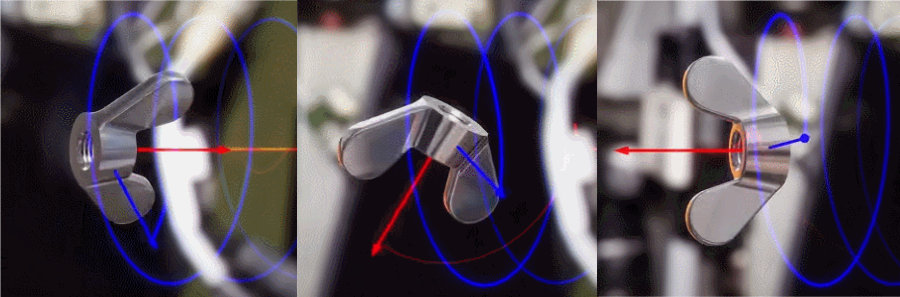
\includegraphics[width=0.9\textwidth]{dzhani.jpg}
\end{center}
   \caption{ภาพแสดงปรากฏการณ์การแกว่งในลักษณะจานิเบคอฟ \cite{28}.}
\label{fig:10}
\end{figure*}

หลักการเบื้องหลังการเปลี่ยนแปลงแกนหมุนของโลกอย่างรวดเร็ว อยู่ที่ฟิสิกส์ของวัตถุหมุน ตัวอย่างมาตรฐานคือปรากฏการณ์การแกว่งในลักษณะจานิเบคอฟ ซึ่งค้นพบโดยนักบินอวกาศชาวรัสเซีย วลาดีมีร์ จานิเบคอฟ \cite{37} และแสดงในรูปที่ \ref{fig:10} วัตถุที่ไม่ได้หมุนอย่างสมบูรณ์บนแกนหลักสามแกนใดแกนหนึ่งของความเฉื่อย จะไม่สามารถรักษาระนาบการหมุนให้คงที่ได้หากวัตถุนั้นหมุนใกล้กับแกนหลักที่สอง และมันจะเกิดสิ่งที่ดูเหมือนเป็นการเปลี่ยนแปลงการหมุนอย่างกะทันหัน แม้ว่าสิ่งนี้จะไม่ใช่สิ่งที่เราเชื่อว่าเกิดขึ้นระหว่างการพลิกกลับอย่างรวดเร็วของโลก แต่ประเด็นคือในกรณีที่ไม่มีแรงภายนอกเข้ามาเกี่ยวข้อง มีเพียงฟิสิกส์ของการหมุนเท่านั้นที่สามารถอธิบายการเปลี่ยนแปลงอย่างรวดเร็วของแกนการหมุนของโลกได้

\begin{figure}[t]
\begin{center}
% \fbox{\rule{0pt}{2in} \rule{0.9\linewidth}{0pt}}
   \includegraphics[width=1\linewidth]{llvp.jpg}
\end{center}
   \caption{ภาพเชิงลึกของ LLVP ใต้แอฟริกาใต้ \cite{28}.}
\label{fig:12}
\label{fig:onecol}
\end{figure}

\begin{figure*}[t]
\begin{center}
% \fbox{\rule{0pt}{2in} \rule{.9\linewidth}{0pt}}
\includegraphics[width=1\textwidth]{layers.jpg}
\end{center}
   \caption{ภาพแสดงกระบวนการภายในโลกที่นำไปสู่การพลิกกลับแบบ ECDO \cite{129}.}
\label{fig:11}
\end{figure*}

เพื่อความแม่นยำ โลกแทบจะไม่ได้เกิดปรากฏการณ์การแกว่งในลักษณะจานิเบคอฟแบบเรียบง่ายและสม่ำเสมอ หากเป็นเช่นนั้น เราต้องสามารถตรวจจับการเปลี่ยนแปลงแกนหมุนของโลกอย่างค่อยเป็นค่อยไปเมื่อเวลาผ่านไป ตรงกันข้าม เราเชื่อว่าโลกประสบกับการหยุดชะงักอย่างกะทันหันเป็นช่วงๆ ในโครงสร้างทางกายภาพของมัน ส่งผลให้เกิดการแยกตัวระหว่าง "ส่วนหมุนรอบนอก" (เปลือกโลก/ เนื้อโลก) และ "ส่วนหมุนรอบใน" (แกนกลาง) ตามกฎการอนุรักษ์โมเมนต์เชิงมุม หากไม่มีแรงกระตุ้นจากภายนอก โลกจะไม่สามารถเปลี่ยนแกนหมุนอย่างทันทีทันใดได้ ดังนั้นการแยกระหว่างวัตถุหมุนชั้นในและชั้นนอกจึงเป็นหนึ่งในไม่กี่สิ่ง (นอกเหนือจากผลกระทบจากภายนอก) ที่อาจทำให้เกิดการกลับแกนหมุนอย่างรวดเร็วและรุนแรง

กระบวนการเฉพาะที่ขับเคลื่อนการหยุดชะงักภายในของโลก เชื่อว่าเป็นการเปลี่ยนสถานะในโครงสร้างของเหล็กที่เป็นองค์ประกอบหลักของแกนโลก (รูปที่ \ref{fig:11}) แกนในประกอบด้วยเหล็กที่มีโครงสร้างผลึกแบบปิดแน่นเชิงหกเหลี่ยม (Fe) \cite{141} เมื่อ เหล็กที่มีโครงสร้างผลึกแบบปิดแน่นเชิงหกเหลี่ยม นี้เปลี่ยนสถานะโลหะเหลว จะปลดปล่อยพลังงานจลน์และถูกเคลื่อนเข้าไปในแกนชั้นนอก การเปลี่ยนสถานะนี้ลดความสามารถในการนำแม่เหล็กของแกนกลาง ทำให้สนามแม่เหล็กโลกอ่อนตัวลง และปลดปล่อยความร้อน สร้างโครงสร้างบริเวณขนาดใหญ่ที่มีความเร็วคลื่นเฉือนต่ำ LLVP (large low-velocity shear province) (รูปที่ \ref{fig:12}) \cite{38} ในชั้นเนื้อโลก และเพิ่มอุณหภูมิพื้นผิวโลกผ่านมหาสมุทรน้ำลึก ทั้งสองแนวโน้มถูกบันทึกไว้อย่างดีในศตวรรษหลัง ๆ และจะมีการกล่าวถึงในส่วนถัดไปของเอกสารนี้



กระบวนการเดียวกันนี้ภายในโลก ซึ่งเกิดขึ้นในทิศทางตรงกันข้าม ยังเชื่อกันว่าเป็นตัวผลักดันให้เกิดการเปลี่ยนกลับสู่สภาวะการหมุนของโลกในรูปแบบปัจจุบันในเวลาไม่นานหลังจากการพลิกกลับเกิดขึ้น

\section{หลักฐานการพลิกตัวของโลกที่กำลังจะเกิดขึ้น}
มีเหตุผลที่แข็งแกร่งที่เชื่อได้ว่าเรากำลังจะถึงการพลิกสลับขั้วแม่เหล็กโลกอีกครั้ง . ยพิบัติไม่ได้เกิดขึ้นมาหลายพันปีแล้ว ยพิบัติไม่ได้เกิดขึ้นมาหลายพันปีแล้ว ข้อมูลที่แข็งแกร่งที่สุดที่สนับสนุนการพลิกตัวที่กำลังจะเกิดขึ้นมาจากข้อมูลแม่เหล็กโลกเมื่อเร็วๆ นี้ ซึ่งบ่งชี้ว่าสนามแม่เหล็กโลกอ่อนแอลงมาประมาณสองพันปีแล้วการอ่อนแอลงนี้เร่งตัวขึ้นและถึงอัตราที่น่าตกใจในช่วงไม่กี่ทศวรรษที่ผ่านมา

แสดงในรูป \ref{fig:14} แสดงสนามแม่เหล็กโลกที่อ่อนแอลงตั้งแต่ปีค.ศ. 1590 ถึง 2025 \cite{125,126}. ดังแสดงในรูปภาพ สนามแม่เหล็กอ่อนแอลงอย่างมีนัยสำคัญ 

อีกหนึ่งตัวชี้วัดสำหรับการอ่อนแอของสนามแม่เหล็กโลกคือตำแหน่งของขั้วแม่เหล็กเหนือ (รูปที่ \ref{fig:13}).  ขั้วแม่เหล็กเหนือ ในอดีตตั้งอยู่ในแถบอาร์กติกของแคนาดา อย่างไรก็ตามมันได้เคลื่อนที่อย่างช้าๆ ตลอดหลายศตวรรษที่ผ่านมา และเร่งตัวขึ้นอย่างมีนัยสำคัญเมื่อไม่กี่ทศวรรษที่ผ่านมา ตอนนี้มันกำลังเคลื่อนที่อย่างรวดเร็วไปยังรัสเซียด้วยอัตรา 55 กิโลเมตรต่อปี \cite{124}.

\begin{figure*}[t]
\begin{center}
% \fbox{\rule{0pt}{2in} \rule{.9\linewidth}{0pt}}
\includegraphics[width=0.9\textwidth]{saa.jpg}
\end{center}
   \caption{ภาพแสดงสนามแม่เหล็กโลกที่อ่อนตัวลงตั้งแต่ปีค.ศ. 1590 ถึง 2025 คำนวณโดยใช้แบบจำลอง gufm1 และ IGRF-14 \cite{125,126}.}
\label{fig:14}
\end{figure*}

\begin{figure}[t]
\begin{center}
% \fbox{\rule{0pt}{2in} \rule{1\linewidth}{0pt}}
   \includegraphics[width=1\linewidth]{npw.jpg}
\end{center}

\caption{ตำแหน่งของขั้วแม่เหล็กโลกเหนือ ตั้งแต่ปีค.ศ. 1590 ถึง 2025 แสดงเป็นช่วงเวลาทีละ 5 ปี \cite{142}.}
\label{fig:13}
\label{fig:onecol}
\end{figure}

\begin{figure}[t]
\begin{center}
% \fbox{\rule{0pt}{2in} \rule{1\linewidth}{0pt}}
   \includegraphics[width=1\linewidth]{ocean-highlight.jpg}
\end{center}
   \caption{อัตราการอุ่นขึ้นของมหาสมุทรส่วนลึก (ลึกกว่า 2000 เมตร) ตั้งแต่ปี 1991 ถึง 2010 ซึ่งถูกวงไว้ด้วยสีแดง \cite{132}.}
\label{fig:15}
\label{fig:onecol}
\end{figure}

สนามแม่เหล็กของโลกเชื่อว่าถูกสร้างขึ้นจากเครื่องกำเนิดสนามแม่เหล็กอยู่ภายในแกนโลก—กระแสแมกมาที่เคลื่อนที่เป็นอยู่ในแก่นโลกชั้นนอกเนื่องจากการหมุนของโลก \cite{123}. การอ่อนกำลังของสนามแม่เหล็กโลกเป็นอาการของการเปลี่ยนแปลงอย่างรุนแรงลึกภายในโลก ตามทฤษฎี ECDO การเปลี่ยนแปลงอย่างรุนแรงเหล่านี้จะทำให้เกิดการปล่อยความร้อน และในที่สุดนำไปสู่การแยกระหว่างเนื้อโลกกับแก่นโลก ส่งผลให้เกิดการพลิกสลับขั้วแม่เหล็กโลก \cite{1}.

มีข้อมูลจำนวนมากที่สนับสนุนการมีอยู่ของกระบวนการเกิดความร้อนภายในโลก ข้อมูลเกี่ยวกับโลกร้อนปรากฏในอุณหภูมิผิวทวีปและมหาสมุทรที่เพิ่มสูงขึ้น \cite{127,128} ระดับก๊าซคาร์บอนไดออกไซด์ในบรรยากาศที่เพิ่มขึ้นสัมพันธ์กับกลุ่มความร้อนของโลก \cite{129,130} และปริมาณน้ำแข็งทะเลทั่วโลกลดลง \cite{131}. ข้อมูลเหล่านี้ชี้ให้เห็นว่าระดับก๊าซคาร์บอนไดออกไซด์ และอุณหภูมิที่สูงขึ้นไม่ใช่สาเหตุของ “การเปลี่ยนแปลงสภาพภูมิอากาศที่มนุษย์สร้างขึ้น” แต่เป็นผลสืบเนื่องจากแก่นโลกที่ปล่อยความร้อนออกมา \cite{129}.

ที่สำคัญที่สุด การศึกษาอัตราการอุ่นขึ้นของมหาสมุทรส่วนลึก (ลึกกว่า 2000 เมตร) แสดงให้เห็นว่าไม่เพียงแต่มหาสมุทรส่วนลึกกำลังร้อนขึ้นแต่อัตราการอุ่นขึ้นที่แรงที่สุดพบในชั้นแอบิสซอล (4000 - 6000 เมตร) โดยศูนย์กลางของการอุ่นนี้อยู่ต่ำกว่า 4000 เมตร \cite{132,129} ซึ่งจะเป็นไปไม่ได้หากมหาสมุทรได้รับความร้อนจากด้านบนโดยบรรยากาศ ข้อมูลเช่นนี้สนับสนุนอย่างมากต่อแนวคิดที่ว่าการเปลี่ยนแปลงด้านภูมิอากาศและสนามแม่เหล็กโลกที่ผ่านมาในปัจจุบัน ขับเคลื่อนโดยกระบวนการที่อยู่ลึกภายในโลก รูปที่ \ref{fig:15} แสดงอัตราการอุ่นขึ้นของมหาสมุทรส่วนลึกทั่วโลก ตั้งแต่ปี 1991 ถึง 2010 \cite{132}.
\section{การสร้างแบบจำลองการพลิกสลับขั้วแม่เหล็กโลกที่กำลังจะมาถึง}

\begin{figure}[b]
\begin{center}
% \fbox{\rule{0pt}{2in} \rule{1\linewidth}{0pt}}
   \includegraphics[width=1\linewidth]{saa-crop.jpeg}
\end{center}
   \caption{การคำนวณจุดพลิกผันโดยอิงจากSouth Atlantic Anomaly ชี้ไปที่วันที่ 13 มีนาคม 2059 \cite{125,126}.}
\label{fig:16}
\label{fig:onecol}
\end{figure}

การคาดการณ์เวลาที่โลกการพลิกสลับขั้วแม่เหล็กโลกครั้งต่อไปเป็นงานที่ซับซ้อน ปัจจุบัน แบบจำลองที่ดีที่สุดที่เรามีสำหรับเรื่องนี้คือสนามแม่เหล็กโลก บริเวณ South Atlantic Anomaly (SAA) พื้นที่นี้ที่อยู่เหนือน่านน้ำแอตแลนติกใต้มีความเข้มสนามแม่เหล็กต่ำที่สุด และถูกกำหนดให้เป็นบริเวณที่มีค่าความเข้มของสนามต่ำกว่า 32,000 นาโนเทสลา \cite{135} ซึ่งเป็นค่าต่ำที่สุดที่เคยบันทึกไว้ในปี 1590 พื้นที่ของ South Atlantic Anomaly มีขนาดเพิ่มขึ้นจาก 1\% ของพื้นผิวโลกในปี 1590 เป็น 21\% ในปี 2025 \cite{136}

เพื่อประมาณการว่าโลกอาจจะพลิกกลับเมื่อใด ผู้เขียนได้นำข้อมูลขอบเขตพื้นผิวของปรากฏการณ์ความผิดปกติของสนามแม่เหล็กโลกแอตแลนติกใต้ (SAA)ให้เข้ากับสมการกฎกำลังและจุดพลิกผันที่เป็นแบบจำลองของระบบซับซ้อนที่เข้าใกล้จุดเปลี่ยนวิกฤต ซึ่งระบบจะเกิดการเปลี่ยนแปลงอย่างรวดเร็วและรุนแรง การคำนวณของผู้เขียนได้ทำนายจุดพลิกผันที่คาดการณ์ไว้คือวันที่ 13 มีนาคม ค.ศ.2059 (ดูรูป \ref{fig:16}) การคาดการณ์นี้จะมีความแม่นยำมากขึ้นเรื่อย ๆ เมื่อเราเข้าใกล้ช่วงเวลาแห่งการเปลี่ยนแปลง \cite{136}

ตัวชี้วัดอื่น ๆ เช่น การเคลื่อนที่ของแกนหมุนของโลก, ความผิดปกติของสภาพอากาศ, และข้อมูลแผ่นดินไหวกับภูเขาไฟ ก็สามารถช่วยให้เราคาดการณ์เวลาที่โลกจะพลิกกลับครั้งต่อไปได้แม่นยำยิ่งขึ้น

\section{เส้นเวลาเหตุการณ์สำคัญของ ECDO}แม้การแสดงลำดับเหตุการณ์ ที่แม่นยำสำหรับเหตุการณ์ ECDO ในอดีตเป็นเรื่องยาก แต่ดูเหมือนว่ามีเหตุการณ์ ECDO อย่างน้อย 2 เรื่องราวที่เฮโรโดตุสได้รับมาจากนักบวชชาวอียิปต์ที่กล่าวว่า
 \textit{"จากกษัตริย์องค์แรกจนถึงนักบวชแห่งเฮเฟสทัสองค์สุดท้าย มีมนุษย์ 341 รุ่น... พวกเขาบอกว่า ดวงอาทิตย์ได้ขยับสี่ครั้งจากจุดที่มันขึ้นประจำ และจากที่ที่มันตกในปัจจุบันมันเคยขึ้นมาแล้วสองครั้ง  และในที่ที่มันขึ้นในปัจจุบัน มันเคยตกมาแล้วสองครั้ง"} \cite{32}. เพลโต ซึ่งมีชีวิตอยู่ในช่วงศตวรรษที่ห้าก่อนคริสต์ศักราช \cite{111} กล่าวว่าหลังจากน้ำท่วมที่จมแอตแลนติสภายในวันเดียว 9,000 ปีก่อน \textit{"ตั้งแต่นั้นเป็นต้นมาได้มีน้ำท่วมใหญ่หลายครั้ง และผู้รอดชีวิตที่พำนักอยู่บนภูเขาไม่รู้จักศิลปะแห่งการเขียน และในหลายชั่วอายุคนก็ทุ่มเทอย่างเต็มที่เพื่อการดำรงชีวิต"} \cite{112} ซึ่งบ่งชี้ว่าอาจมีการพลิกสลับขั้วแม่เหล็กโลกมากกว่าสองครั้งตั้งแต่สิ้นสุดยุค Younger Dryas ประมาณ 9,700 ปีก่อนคริสต์ศักราช หลักฐานทางกายภาพที่นำเสนอตลอดบทความนี้และในการวิจัยของผู้เขียน \cite{2} เป็นหลักฐานที่เพียงพอสำหรับเรื่องเล่าของเพลโต

วันที่ที่คาดว่าเกิดการพลิกสลับขั้วแม่เหล็กโลก แบบECDO ล่าสุดคือช่วงปี 2300 ถึง 1600 ก่อนคริสต์ศักราช ซึ่งตำนานอุทกภัยครั้งใหญ่หลายกรณี (กุ่นอวี่ \cite{113,114,115}, น้ำท่วมออกิกีส \cite{116,117}, เปรู \cite{118,119}, การอพยพ \cite{120}), การล่มสลายและการละทิ้งอารยธรรม (โมเฮนโจดาโร \cite{121}, อารยธรรมไมนอสในครีต \cite{100,101}) และความผิดปกติทางกายภาพ (ปรากฏการณ์บอนด์ \cite{122}, เหตุการณ์ 4.2 พันปี \cite{90}) ได้ถูกลงวันที่ ยังไม่มีหลักฐานมาบรรจบกันอย่างเพียงพอที่ใหม่กว่านี้ซึ่งชี้ให้เห็นถึงเหตุการณ์ภัยพิบัติใหญ่

\section{บทสรุป}

ปฏิบัติการ NANOOK เป็นความพยายามลาดตระเวนในช่วงสงครามเย็นของสหรัฐอเมริกา เพื่อแผนที่ขั้วโลกเหนือและชายฝั่งโซเวียตตอนเหนือหลังสงครามโลกครั้งที่สอง \cite{137} ในระหว่างการสืบสวน พวกเขาค้นพบว่าขั้วแม่เหล็กอยู่ห่างออกไป 125 ถึง 200 ไมล์ ทางเหนือจากตำแหน่งที่ควรจะเป็น โดยอิงจากการค้นพบจากการสำรวจก่อนหน้านี้ ดังนั้น\textit{"ในหมู่นักวิทยาศาสตร์รัฐบาล จึงเกิดคำถามขึ้นมาว่าจะเกิดอะไรขึ้นเมื่อขั้วแม่เหล็กโลกกับขั้วทางภูมิศาสตร์มาตรงกัน เพื่อหาคำตอบนี้ ภายใต้การควบคุมโครงการของ ดร. พอล เอ. ไซเปิล บริษัทแรนด์คอร์ปอเรชั่นได้รับสัญญาให้ทำการทดลองในห้องปฏิบัติการโดยใช้แบบจำลองโลกที่สร้างจากทรงกลมซ้อนกัน – ทรงกลมด้านในแทนแกนเหล็กหลอมเหลวที่ประจุไฟฟ้าแม่เหล็กของโลกซึ่งแกนโลกเป็น “ขั้วแม่เหล็ก” ; และทรงกลมด้านนอกแทนเปลือกโลกที่หมุนรอบแกนขั้วโลกทาง “ภูมิศาสตร์” เมื่อมีการพิจารณาจากการทดลองซ้ำๆ พบว่าเมื่อขั้ว  “แม่เหล็ก” เคลื่อนเข้าใกล้ขั้ว “ภูมิศาสตร์” ขั้วแม่เหล็กจะเร่งความเร็วในการเคลื่อนเข้าใกล้อย่างรุนแรงเหมือนถูกดึงด้วยแรงเหวี่ยงเข้าสู่ขั้วภูมิศาสตร์และเคลื่อนไปตรงกันในที่สุด แต่แทนที่จะซ้อนตรงกัน ขั้ว “แม่เหล็ก” จะ “พลิก” อย่างรวดเร็วไปรอบขั้ว “ภูมิศาสตร์” และยิงออกไปทางเส้นศูนย์สูตรเหมือนกับแรงเหวี่ยง จนจบลงที่ตำแหน่งที่มุมสองแกนแยกกันประมาณ 89 องศา หลังการ “พลิก” ของขั้วนี้เกิดขึ้นแล้ว แกนทั้งสองจะเริ่มกลับเข้าหากันอย่างช้าๆ ตลอดเวลาที่ยาวนาน"} \cite{138,139}

ต่อมา \textit{"ที่การประชุมวิทยาศาสตร์ที่พันตรีไวท์เข้าร่วมหนึ่งในอาคารเพนตากอนช่วงต้นปี 1948 เหล่านักวิทยาศาสตร์ได้ถกเถียงกันถึงความเหมาะสมในการเตือนสาธารณชนเกี่ยวกับปรากฏการณ์การพลิกสลับขั้วแม่เหล็กโลกนี้ ไม่มีนักวิทยาศาสตร์คนใดเห็นควรจะปิดบังข้อมูลจากสาธารณะ แต่ในทางกลับกัน ก็ไม่มีใครตกลงกันได้ว่าจะเปิดเผยข้อมูลอย่างไร ความรู้นี้ บางคนคิดว่า อาจจะทำลายจิตวิญญาณทางจริยธรรมของสังคมด้วยซ้ำ ทว่าความกลัวนี้ดูจะไม่มีมูล เมื่อในต้นทศวรรษ 1950 ข้อมูลเกี่ยวกับปรากฏการณ์ขั้วโลกพลิกถูกเผยแพร่ทั้งในคอลัมน์หนังสือพิมพ์และบทความนิตยสาร แต่กลับไม่เกิดการตอบรับใด ๆ จากสาธารณชนที่ดูเหมือนจะตะลึงงันหรือไม่เชื่อ"} \cite{138,139}

ทำไมเราถึงไม่ใส่ใจกับเรื่องนี้? มีเหตุผลมากมายที่เชื่อว่าโลกเคยพลิกกลับมาก่อน เอกสารนี้ พร้อมกับตอนที่สองของบทความนี้ สรุปหลักฐานจำนวนมหาศาลจากหลากหลายแขนงที่บ่งชี้ว่าสิ่งนี้เป็นความจริง เช่น ตำนานน้ำท่วมทั่วโลก เกลือและฟอสซิลทะเลที่ปกคลุมพื้นทวีป ที่หลบภัยใต้ดินโบราณ ซากสัตว์ และภูมิทัศน์ทางธรณีวิทยาที่เกิดจากภัยพิบัติ มนุษย์มีอายุหลายแสนปีโดยประมาณ แต่ประวัติศาสตร์สมัยใหม่ของเรามีแค่ไม่กี่พันปี อาจเป็นไปได้ไหมว่าทุก ๆ ระยะหนึ่ง โลกจะพลิกสลับขั้วแม่เหล็กโลก ทวีปถูกล้างจนเกลี้ยง แล้วเราก็ต้องกลับไปเริ่มต้นใหม่เหมือนยุคหิน ลดบันทึกประวัติศาสตร์โบราณเหลือเพียงเรื่องเล่าภัยพิบัติไม่กี่เรื่อง หากเป็นเช่นนั้น การป้องกันไม่ให้มันเกิดขึ้นอีกก็อาจเป็นภารกิจสำคัญที่สุดของมนุษยชาติ

สุดท้ายนี้ ผู้เขียนขอฝากบัญชีเรื่องเล่าที่ถูกบันทึกไว้ในหนังสือ Timaeus โดยเพลโต เกี่ยวกับการพูดคุยระหว่างโซลอน (Solon) นักการเมืองชาวเอเธนส์และนักบวชชาวอียิปต์ \cite{140}: \textit{"วันหนึ่ง เมื่อ [โซลอน] ต้องการชักชวนให้นักบวชสนทนาเรื่องประวัติศาสตร์โบราณ เขาเล่าขนบธรรมเนียมที่เก่าแก่ที่สุดของเราเกี่ยวกับฟอโรเนอุส (Phoroneus) ซึ่งเชื่อกันว่าเป็นมนุษย์คนแรก และนิโอเบ แล้วเขาก็เล่าตำนานเกี่ยวกับเดอูคาเลียนและพีร์รา (Deucalion and Pyrrha) หลังน้ำท่วม และว่าพวกเขารอดมาได้อย่างไร รวมถึงบอกสายตระกูลของลูกหลานพวกเขา และด้วยการบอกจำนวนปีที่เหตุการณ์เหล่านั้นเกิดขึ้น เขาพยายามคำนวณระยะเวลา โดยขณะนั้นนักบวชคนหนึ่งที่แก่ชรามากกล่าวขึ้นว่า “โอ้ โซลอน โซลอน ชาวกรีกทั้งหลายยังเป็นเด็กอยู่เสมอ ไม่เคยมีชาวกรีกคนใดแก่เลย” เมื่อได้ยินเช่นนี้เขาจึงถามว่า “ท่านหมายความว่าอย่างไร?” นักบวชจึงตอบว่า “พวกท่านยังเด็กในจิตวิญญาณ ทุกคนเลย เพราะว่าพวกท่านไม่มีความเชื่อหรือภูมิปัญญาใด ๆ ที่ได้รับตกทอดมาแต่โบราณ และไม่รู้วิทยาการใดที่เก่าแก่ จริง ๆ แล้วเหตุที่เป็นเช่นนี้ก็เพราะมีการทำลายล้างมนุษยชาติมากมายหลายรูปแบบทั้งที่เกิดขึ้นแล้วและกำลังจะเกิดขึ้น ท้จริงแล้ว เรื่องเล่าที่เล่าขานกันในประเทศของคุณและของเรา ที่ว่าครั้งหนึ่งนานมาแล้ว เฟธอน บุตรชายของเฮลิออส ได้บังคับราชรถของบิดา และเพราะไม่สามารถขับขี่ไปตามเส้นทางที่บิดาเคยขับได้ จึงเผาผลาญทุกสิ่งบนโลก และตัวเขาเองก็ดับดิ้นด้วยอสุนีบาต — เรื่องเล่านั้น ตามที่เล่าขานกัน มีลักษณะเป็นตำนาน แต่ความจริงของมันอยู่ที่การเกิดการเคลื่อนที่ของวัตถุบนท้องฟ้าที่โคจรรอบโลก และการทำลายล้างสิ่งต่าง ๆ บนโลกด้วยไฟอันรุนแรง ซึ่งเกิดขึ้นซ้ำ ๆ หมุนเวียนมาเป็นระยะ ๆ  ในเวลาเช่นนั้น ผู้ที่อาศัยอยู่บนภูเขาและในที่สูงและแห้งแล้งต้องประสบกับการทำลายล้างมากกว่าผู้ที่อาศัยอยู่ใกล้แม่น้ำหรือทะเล; และในกรณีของเรา แม่น้ำไนล์ ซึ่งเป็นผู้กอบกู้เราในทางอื่น ๆ ก็ช่วยเราให้พ้นจากภัยพิบัตินี้ด้วยการขึ้นสูง และเมื่ออีกด้านหนึ่ง เหล่าทวยเทพชำระล้างโลกด้วยน้ำท่วม คนที่ดูแลฝูงสัตว์และคนเลี้ยงแกะที่อยู่บนภูเขาทุกคนก็รอดชีวิต แต่ผู้ที่อยู่ในเมืองของคุณถูกกระแสน้ำพัดพาลงสู่ทะเล; ในขณะที่ประเทศของเรา ไม่ว่าจะเป็นในเวลานั้นหรือเวลาอื่น ๆ น้ำก็ไม่เคยหลากท่วมทุ่งนาของเราจากเบื้องบนเลย ตรงกันข้าม น้ำทั้งหมดมักจะผุดขึ้นมาจากเบื้องล่างตามธรรมชาติ ด้วยเหตุผลเหล่านี้เอง สิ่งที่ได้รับการอนุรักษ์ไว้ที่นี่จึงถือว่าเก่าแก่ที่สุด ความจริงคือในทุก ๆ ที่ที่ไม่มีความร้อนจัดหรือความเย็นจัดเกินไปจนขัดขวาง ก็มักจะมีเผ่าพันธุ์มนุษย์อยู่เสมอ ไม่ว่าจะมีจำนวนมากหรือน้อย และหากมีเหตุการณ์ใด ๆ เกิดขึ้นที่สูงส่ง ยิ่งใหญ่ หรือเด่นชัดไม่ว่าด้วยวิธีใด ไม่ว่าจะเป็นในประเทศของคุณ หรือในประเทศของเรา หรือในที่อื่นใดที่เราทราบจากรายงาน เหตุการณ์เหล่านั้นล้วนถูกบันทึกไว้ตั้งแต่สมัยโบราณและเก็บรักษาไว้ที่นี่ในวิหารของเรา; ในขณะที่ผู้คนของคุณและคนอื่น ๆ เพิ่งได้รับการจัดเตรียมด้วยตัวอักษรและศิลปะต่าง ๆ ที่รัฐที่เจริญแล้วต้องการ และเมื่อหลังจากช่วงเวลาหลายปีตามปกติ เหมือนโรคระบาด น้ำท่วมจากฟากฟ้าก็พัดถล่มผู้คนของคุณอีกครั้ง มันไม่เหลือใครนอกจากผู้ที่ไร้การศึกษาและไม่มีวัฒนธรรม ทำให้คุณกลับมาเยาว์วัยเช่นเดิม โดยไม่มีความรู้เกี่ยวกับสิ่งที่เกิดขึ้นในอดีตในดินแดนนี้หรือในดินแดนของคุณ แน่นอนว่าลำดับวงศ์ตระกูลที่คุณเล่าเมื่อครู่นี้ โซลอน เกี่ยวกับผู้คนในประเทศของคุณ แทบจะดีกว่านิทานเด็กเล็ก ๆ เสียอีก; ประการแรก คุณจำได้เพียงน้ำท่วมครั้งเดียว ทั้งที่มีหลายครั้งเกิดขึ้นก่อนหน้านั้น; และประการถัดไป คุณไม่ทราบความจริงที่ว่าเผ่าพันธุ์ที่สูงส่งและสมบูรณ์แบบที่สุดในหมู่มนุษย์ถือกำเนิดขึ้นในดินแดนที่คุณอาศัยอยู่ในปัจจุบัน และจากพวกเขา ทั้งตัวคุณเองและเมืองที่คุณมีอยู่ทั้งหมดก็สืบเชื้อสายมาจากเมล็ดพันธุ์เล็ก ๆ ที่บังเอิญเหลือรอด; แต่สิ่งนี้กลับรอดพ้นความสังเกตของคุณไป เพราะหลายชั่วอายุคน ผู้รอดชีวิตได้เสียชีวิตไปโดยไม่มีอำนาจที่จะแสดงออกเป็นลายลักษณ์อักษร เพราะแท้จริงแล้ว ครั้งหนึ่ง โซลอน ก่อนการทำลายล้างครั้งใหญ่ที่สุดด้วยน้ำ สิ่งที่ปัจจุบันคือรัฐเอเธนส์เป็นรัฐที่กล้าหาญที่สุดในสงครามและมีการจัดการที่ดีเยี่ยมในทุกด้านด้วยเช่นกัน กล่าวกันว่ารัฐนี้มีงานศิลปะที่งดงามที่สุดและการปกครองที่สูงส่งที่สุดในบรรดาชนชาติใด ๆ ใต้ฟ้านี้เท่าที่เราเคยได้ยินมา"}.

นักบวชกลุ่มเดียวกันนี้เอง ได้เล่าให้โซลอนฟังถึงอารยธรรมโบราณของแอตแลนติสว่า: \textit{"เพราะทุกสิ่งที่เรามีอยู่ที่นี่ ซึ่งอยู่ภายในช่องปากที่เรากล่าวถึงนั้น เห็นได้ชัดว่าเป็นอ่าวที่มีทางเข้าแคบ; แต่ที่อยู่ไกลออกไปนั้นคือมหาสมุทรที่แท้จริง และดินแดนที่ล้อมรอบมันอาจเรียกได้อย่างถูกต้องที่สุด ในความหมายที่สมบูรณ์และแท้จริง ว่าเป็นทวีป ตอนนี้ในเกาะแอตแลนติสแห่งนี้ มีสมาพันธ์กษัตริย์ที่มีอำนาจยิ่งใหญ่และน่าอัศจรรย์ ซึ่งปกครองเหนือเกาะทั้งหมด และเหนือเกาะอื่นๆ อีกมากมาย รวมถึงบางส่วนของทวีป; ยิ่งไปกว่านั้น จากดินแดนภายในช่องแคบ พวกเขาปกครองลิเบียไปจนถึงอียิปต์ และปกครองยุโรปไปจนถึงไทร์ริเนีย ดังนั้น กองทัพนี้ เมื่อรวมตัวกันทั้งหมด จึงพยายามที่จะเข้ายึดครองประเทศของคุณและของเรา รวมถึงอาณาเขตทั้งหมดภายในช่องแคบด้วยการโจมตีเพียงครั้งเดียว และในเวลานั้นเอง โซลอน ความกล้าหาญและความแข็งแกร่งของบุรุษเพศแห่งรัฐของคุณได้แสดงออกอย่างโดดเด่นต่อสายตาชาวโลก เพราะมันโดดเด่นเหนือสิ่งอื่นใดในด้านความกล้าหาญและศิลปะการทำสงครามทั้งหมด และการกระทำบางส่วนในฐานะผู้นำของชาวกรีก และบางส่วนยืนหยัดอยู่ตามลำพังเมื่อถูกทอดทิ้งโดยคนอื่นๆ หลังจากเผชิญหน้ากับภยันตรายร้ายแรงที่สุด มันได้เอาชนะผู้รุกรานและตั้งอนุสาวรีย์แห่งชัยชนะ; ด้วยเหตุนี้ มันจึงช่วยผู้ที่ยังไม่ตกเป็นทาสให้พ้นจากความเป็นทาส และปลดปล่อยพวกเราที่เหลือทั้งหมดที่อาศัยอยู่ภายในเขตแดนของเฮอร์คิวลีสอย่างไม่เสียดาย แต่ต่อมาเกิดแผ่นดินไหวและน้ำท่วมครั้งใหญ่ และวันคืนอันน่าเศร้าโศกได้มาเยือนพวกเขา เมื่อร่างของนักรบของคุณทั้งหมดถูกกลืนหายไปใต้พื้นโลก และเกาะแอตแลนติสก็ถูกกลืนหายไปใต้ทะเลและอันตรธานไปเช่นกัน"}.

\section{กิตติกรรมประกาศ}

ขอขอบคุณ Ethical Skeptic ผู้เขียนต้นฉบับของวิทยานิพนธ์ ECDO สำหรับการจัดทำวิทยานิพนธ์ที่ลึกซึ้งและบุกเบิกขึ้นมา พร้อมแบ่งปันให้กับโลก วิทยานิพนธ์ทั้งสามส่วนของเขา \cite{1} ยังคงเป็นงานอ้างอิงหลักสำหรับทฤษฎีการแยกตัวของแก่นโลกและเนื้อโลกซึ่งเป็นกระบวนการคายความร้อนทำให้เกิดการแกว่งในลักษณะจานิเบคอฟในการหมุนของโลก(ECDO) และมีข้อมูลเกี่ยวกับหัวข้อนี้มากกว่าที่ข้าพเจ้าได้สรุปไว้โดยสังเขปที่นี่

และแน่นอน ขอบคุณและแสดงความเคารพต่อบุคคลทั้งหลายที่เป็นรากฐานความรู้ให้พัฒนาต่อไป; ผู้ซึ่งได้ทำการวิจัยและสืบสวนทั้งหมดจนทำให้งานนี้บังเกิดขึ้นได้และทำงานเพื่อนำแสงสว่างมาสู่มนุษยชาติ

\clearpage
\twocolumn

\section{ภาพเพิ่มเติม}

\vspace{4cm}

\begin{figure}[htbp]
\begin{center}
% \fbox{\rule{0pt}{2in} \rule{1\linewidth}{0pt}}
   \includegraphics[width=1\linewidth]{wave.jpg}
\end{center}
   \caption{แสดงรายละเอียดเกี่ยวกับรอยสึกกร่อนของคลื่นรูปพาราโบลาที่ถูกกัดเซาะใต้ฐานพีระมิดคาเฟร \cite{27}.}
\label{fig:19}
\label{fig:onecol}
\end{figure}

\begin{figure}[]
\begin{center}
% \fbox{\rule{0pt}{2in} \rule{1\linewidth}{0pt}}
   \includegraphics[width=1\linewidth]{star-stone.jpg}
\end{center}
   \caption{แผนที่ดวงดาวที่แกะสลักลงบนหินในปล่องหนึ่งของพีระมิดคูฟู \cite{28}.}
\label{fig:20}
\label{fig:onecol}
\end{figure}

\clearpage
\twocolumn

\begin{figure*}[t]
\begin{center}
% \fbox{\rule{0pt}{2in} \rule{.9\linewidth}{0pt}}
\includegraphics[width=1\textwidth]{deepsea.jpg}
\end{center}
   \caption{ภาพแสดงความผิดปกติของความร้อนในมหาสมุทรลึกและช่วงก้นสมุทรเมื่อเทียบกับเส้นโค้งความร้อนในมหาสมุทรตามปกติจากชั้นบรรยากาศ ความผิดปกติของความร้อนโดยรวมได้มาจาก NOAA \cite{147} การกระจายความร้อนในระดับลึกและก้นสมุทรจากงานวิจัยของ Desbruyeres \cite{132} และการประมวลผลข้อมูลและการสร้างภาพโดย Ethical Skeptic \cite{129}.}
\label{fig:21}
\end{figure*}

\begin{figure*}[t]
\begin{center}
% \fbox{\rule{0pt}{2in} \rule{.9\linewidth}{0pt}}
\includegraphics[width=1\textwidth]{sealevel.jpeg}
\end{center}
   \caption{ระดับน้ำทะเลแสดงการเพิ่มขึ้นของความแปรปรวน 20\% ในระยะเวลา 75 ปี ที่สถานีตรวจวัด  63 แห่ง บ่งชี้ถึงการเพิ่มขึ้นของความเร็วกระแสน้ำ การพุ่งขึ้นของความแปรปรวนระดับน้ำทะเลเกิดขึ้นพร้อมกับการพุ่งของคลื่นความร้อนในมหาสมุทร บ่งชี้ว่าทั้งสองอาจมีสาเหตุมาจากความร้อนจากส่วนลึกใต้มหาสมุทรของโลก \cite{2,129}.}
\label{fig:22}
\end{figure*}

\begin{figure*}[t]
\begin{center}
% \fbox{\rule{0pt}{2in} \rule{.9\linewidth}{0pt}}
\includegraphics[width=1\textwidth]{co2.jpg}
\end{center}
   \caption{ปริมาณ CO2 ในบรรยากาศ (ppm) เพิ่มขึ้นอย่างต่อเนื่องตลอด 45 ปีที่ผ่านมา  มีแนวโน้มสาเหตุจากอุณหภูมิของมหาสมุทรที่เพิ่มขึ้น ที่มา: NOAA \cite{148,129}.}
\label{fig:23}
\end{figure*}

\begin{figure*}[t]
\begin{center}
% \fbox{\rule{0pt}{2in} \rule{.9\linewidth}{0pt}}
\includegraphics[width=1\textwidth]{ice.jpg}
\end{center}
   \caption{พื้นที่น้ำแข็งทะเลทั่วโลกได้หดตัวลงตลอดในช่วง 45 ปีที่ผ่านมา เนื่องจากโลกร้อนขึ้น แหล่งที่มา: ADS \cite{149}.}
\label{fig:24}
\end{figure*}

\clearpage
\twocolumn

{\small
\bibliographystyle{ieee}
\bibliography{egbib}
}

\end{document}